\documentclass[12pt]{article}
\usepackage{tikz}
\usepackage{amsmath}
% Underlining package
\usepackage{ulem}
\usetikzlibrary{calc}
\usetikzlibrary{angles,quotes}
\usetikzlibrary{decorations.markings, arrows.meta}
\usepackage[a4paper, portrait, margin=1cm]{geometry}
\usepackage{fancyhdr}

\newcommand{\HeadingAnswers}{%
\section*{\Large Name: \underline{\hspace{8cm}} \hfill Date: \underline{\hspace{3cm}}}%
\vspace{-3mm}\par
\textbf{Area Rectangles: Answers}\vspace{1pt}\hrule
}

% raise footer with page number; no header
\fancypagestyle{myfancypagestyle}{
  \fancyhf{}% clear all header and footer fields
  \renewcommand{\headrulewidth}{0pt} % no rule under header
  \fancyfoot[C] {\thepage} \setlength{\footskip}{14.5pt} % raise page number allowed min 14.5pt
}
\pagestyle{myfancypagestyle}  % apply myfancypagestyle

\newcounter{minipagecount}

\begin{document}
\HeadingAnswers
\vspace{8mm}

\begin{minipage}{0.55\textwidth}
  \refstepcounter{minipagecount}
  \noindent{(\theminipagecount)}\quad
 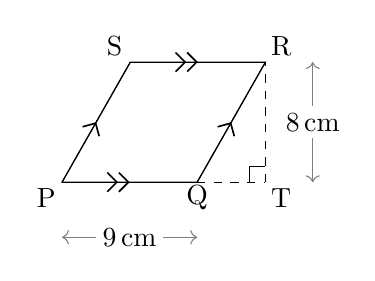
\begin{tikzpicture}[scale=1.0, baseline=(current bounding box.north)]
        \begin{scope}[rotate=0]

       \coordinate (P) at (0,0);
        \coordinate (Q) at (1.716,0);
        \coordinate (T) at ($(Q)+(0.867,0)$);  % extend out
        \coordinate (R) at ($(Q)+(0.867,1.525)$); % Perpendicular upwards
        \coordinate (S) at ($(P)+(0.867,1.525)$); % Perpendicular upwards

        \draw (P)--(Q)--(R)--(S)--cycle;
        \draw[dashed] (Q)--(T);
        \draw[dashed] (T)--(R);

        \pic [draw, -, angle radius=0.2cm] {right angle=Q--T--R};

        \draw[>=Straight Barb, postaction={decorate}, decoration={markings, mark=at position 0.5 with {\arrow[scale=1.5]{>>}}}] (P)--(Q);
        \draw[>=Straight Barb, postaction={decorate}, decoration={markings, mark=at position 0.5 with {\arrow[scale=1.5]{>>}}}] (S)--(R);
        \draw[>=Straight Barb, postaction={decorate}, decoration={markings, mark=at position 0.5 with {\arrow[scale=1.5]{>}}}] (Q)--(R);
        \draw[>=Straight Barb, postaction={decorate}, decoration={markings, mark=at position 0.5 with {\arrow[scale=1.5]{>}}}] (P)--(S);



        % Vertex LABELS
        % Labels relative to shape geometry
        \node at ($(P)+(-0.2,-0.2)$) {P};
        \node at ($(Q)+(0.0,-0.2)$) {Q};
        \node at ($(T)+(0.2,-0.2)$) {T};
        \node at ($(R)+(0.2,0.2)$) {R};
        \node at ($(S)+(-0.2,0.2)$) {S};


        % dotted/dashed arrows shifted away from edges
        % Horizontal side (A-B), shifted down yshift=0mm,
        \draw[<->, gray]
            ($(P) + (0,-0.7cm)$) -- ($(Q) + (0,-0.7cm)$)
            node[black, midway, fill=white, inner sep=2.5pt] {9\,cm};

        % Vertical side (D-C), shifted right xshift=0mm,
        \draw[<->, gray]
            ($(T)+(0.6,0)$) -- ($(T |- R)+(0.6,0)$)
            node[black, midway, fill=white, inner sep=2.5pt] {8\,cm};

    \end{scope}
\end{tikzpicture}
\end{minipage}%
\hfill
\begin{minipage}{.4\textwidth}
  \begin{align*}
    \text{Area} &= \text{bh} \\
    \text{Area} &= 9 \text{cm} \times 8 \text{cm}  \\
    \text{Area} &= 72 \text{cm}^2
  \end{align*}
\end{minipage}

\par\vspace{1cm}\begin{minipage}{0.55\textwidth}
  \refstepcounter{minipagecount}
  \noindent{(\theminipagecount)}\quad
 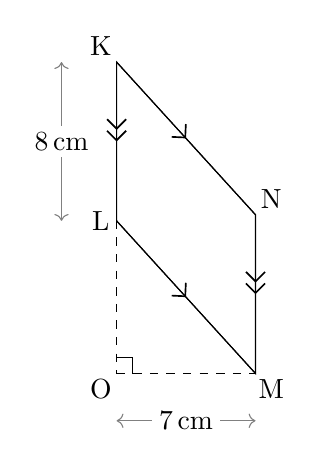
\begin{tikzpicture}[scale=1.0, baseline=(current bounding box.north)]
        \begin{scope}[rotate=270]

       \coordinate (K) at (0,0);
        \coordinate (L) at (2.016,0);
        \coordinate (O) at ($(L)+(1.939,0)$);  % extend out
        \coordinate (M) at ($(L)+(1.939,1.764)$); % Perpendicular upwards
        \coordinate (N) at ($(K)+(1.939,1.764)$); % Perpendicular upwards

        \draw (K)--(L)--(M)--(N)--cycle;
        \draw[dashed] (L)--(O);
        \draw[dashed] (O)--(M);

        \pic [draw, -, angle radius=0.2cm] {right angle=L--O--M};

        \draw[>=Straight Barb, postaction={decorate}, decoration={markings, mark=at position 0.5 with {\arrow[scale=1.5]{>>}}}] (K)--(L);
        \draw[>=Straight Barb, postaction={decorate}, decoration={markings, mark=at position 0.5 with {\arrow[scale=1.5]{>>}}}] (N)--(M);
        \draw[>=Straight Barb, postaction={decorate}, decoration={markings, mark=at position 0.5 with {\arrow[scale=1.5]{>}}}] (L)--(M);
        \draw[>=Straight Barb, postaction={decorate}, decoration={markings, mark=at position 0.5 with {\arrow[scale=1.5]{>}}}] (K)--(N);



        % Vertex LABELS
        % Labels relative to shape geometry
        \node at ($(K)+(-0.2,-0.2)$) {K};
        \node at ($(L)+(0.0,-0.2)$) {L};
        \node at ($(O)+(0.2,-0.2)$) {O};
        \node at ($(M)+(0.2,0.2)$) {M};
        \node at ($(N)+(-0.2,0.2)$) {N};


        % dotted/dashed arrows shifted away from edges
        % Horizontal side (A-B), shifted down yshift=0mm,
        \draw[<->, gray]
            ($(K) + (0,-0.7cm)$) -- ($(L) + (0,-0.7cm)$)
            node[black, midway, fill=white, inner sep=2.5pt] {8\,cm};

        % Vertical side (D-C), shifted right xshift=0mm,
        \draw[<->, gray]
            ($(O)+(0.6,0)$) -- ($(O |- M)+(0.6,0)$)
            node[black, midway, fill=white, inner sep=2.5pt] {7\,cm};

    \end{scope}
\end{tikzpicture}
\end{minipage}%
\hfill
\begin{minipage}{.4\textwidth}
  \begin{align*}
    \text{Area} &= \text{bh} \\
    \text{Area} &= 8 \text{cm} \times 7 \text{cm}  \\
    \text{Area} &= 56 \text{cm}^2
  \end{align*}
\end{minipage}

\par\vspace{1cm}\begin{minipage}{0.55\textwidth}
  \refstepcounter{minipagecount}
  \noindent{(\theminipagecount)}\quad
 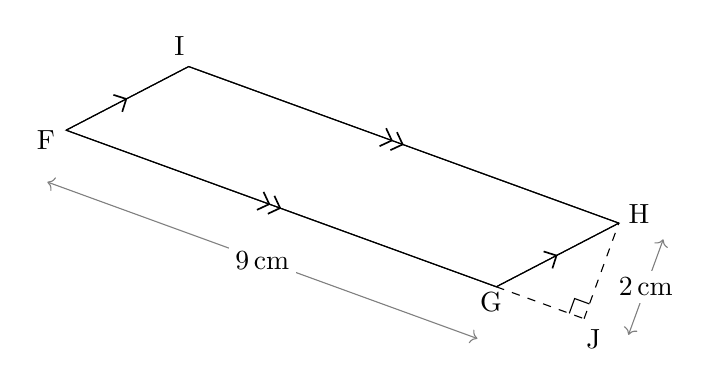
\begin{tikzpicture}[scale=1.0, baseline=(current bounding box.north)]
        \begin{scope}[rotate=-20]

       \coordinate (F) at (0,0);
        \coordinate (G) at (5.814,0);
        \coordinate (J) at ($(G)+(1.186,0)$);  % extend out
        \coordinate (H) at ($(G)+(1.186,1.292)$); % Perpendicular upwards
        \coordinate (I) at ($(F)+(1.186,1.292)$); % Perpendicular upwards

        \draw (F)--(G)--(H)--(I)--cycle;
        \draw[dashed] (G)--(J);
        \draw[dashed] (J)--(H);

        \pic [draw, -, angle radius=0.2cm] {right angle=G--J--H};

        \draw[>=Straight Barb, postaction={decorate}, decoration={markings, mark=at position 0.5 with {\arrow[scale=1.5]{>>}}}] (F)--(G);
        \draw[>=Straight Barb, postaction={decorate}, decoration={markings, mark=at position 0.5 with {\arrow[scale=1.5]{>>}}}] (I)--(H);
        \draw[>=Straight Barb, postaction={decorate}, decoration={markings, mark=at position 0.5 with {\arrow[scale=1.5]{>}}}] (G)--(H);
        \draw[>=Straight Barb, postaction={decorate}, decoration={markings, mark=at position 0.5 with {\arrow[scale=1.5]{>}}}] (F)--(I);



        % Vertex LABELS
        % Labels relative to shape geometry
        \node at ($(F)+(-0.2,-0.2)$) {F};
        \node at ($(G)+(0.0,-0.2)$) {G};
        \node at ($(J)+(0.2,-0.2)$) {J};
        \node at ($(H)+(0.2,0.2)$) {H};
        \node at ($(I)+(-0.2,0.2)$) {I};


        % dotted/dashed arrows shifted away from edges
        % Horizontal side (A-B), shifted down yshift=0mm,
        \draw[<->, gray]
            ($(F) + (0,-0.7cm)$) -- ($(G) + (0,-0.7cm)$)
            node[black, midway, fill=white, inner sep=2.5pt] {9\,cm};

        % Vertical side (D-C), shifted right xshift=0mm,
        \draw[<->, gray]
            ($(J)+(0.6,0)$) -- ($(J |- H)+(0.6,0)$)
            node[black, midway, fill=white, inner sep=2.5pt] {2\,cm};

    \end{scope}
\end{tikzpicture}
\end{minipage}%
\hfill
\begin{minipage}{.4\textwidth}
  \begin{align*}
    \text{Area} &= \text{bh} \\
    \text{Area} &= 9 \text{cm} \times 2 \text{cm}  \\
    \text{Area} &= 18 \text{cm}^2
  \end{align*}
\end{minipage}

\par\vspace{1cm}\begin{minipage}{0.55\textwidth}
  \refstepcounter{minipagecount}
  \noindent{(\theminipagecount)}\quad
 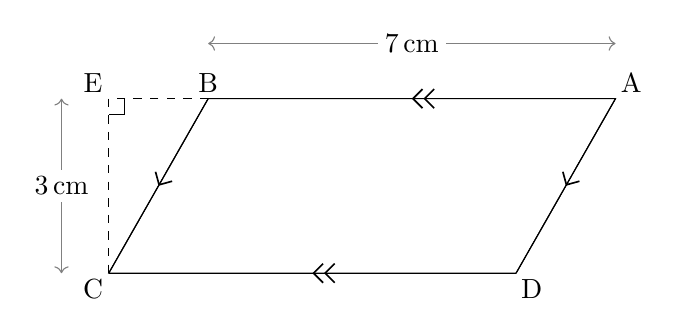
\begin{tikzpicture}[scale=1.0, baseline=(current bounding box.north)]
        \begin{scope}[rotate=180]

       \coordinate (A) at (0,0);
        \coordinate (B) at (5.173,0);
        \coordinate (E) at ($(B)+(1.263,0)$);  % extend out
        \coordinate (C) at ($(B)+(1.263,2.217)$); % Perpendicular upwards
        \coordinate (D) at ($(A)+(1.263,2.217)$); % Perpendicular upwards

        \draw (A)--(B)--(C)--(D)--cycle;
        \draw[dashed] (B)--(E);
        \draw[dashed] (E)--(C);

        \pic [draw, -, angle radius=0.2cm] {right angle=B--E--C};

        \draw[>=Straight Barb, postaction={decorate}, decoration={markings, mark=at position 0.5 with {\arrow[scale=1.5]{>>}}}] (A)--(B);
        \draw[>=Straight Barb, postaction={decorate}, decoration={markings, mark=at position 0.5 with {\arrow[scale=1.5]{>>}}}] (D)--(C);
        \draw[>=Straight Barb, postaction={decorate}, decoration={markings, mark=at position 0.5 with {\arrow[scale=1.5]{>}}}] (B)--(C);
        \draw[>=Straight Barb, postaction={decorate}, decoration={markings, mark=at position 0.5 with {\arrow[scale=1.5]{>}}}] (A)--(D);



        % Vertex LABELS
        % Labels relative to shape geometry
        \node at ($(A)+(-0.2,-0.2)$) {A};
        \node at ($(B)+(0.0,-0.2)$) {B};
        \node at ($(E)+(0.2,-0.2)$) {E};
        \node at ($(C)+(0.2,0.2)$) {C};
        \node at ($(D)+(-0.2,0.2)$) {D};


        % dotted/dashed arrows shifted away from edges
        % Horizontal side (A-B), shifted down yshift=0mm,
        \draw[<->, gray]
            ($(A) + (0,-0.7cm)$) -- ($(B) + (0,-0.7cm)$)
            node[black, midway, fill=white, inner sep=2.5pt] {7\,cm};

        % Vertical side (D-C), shifted right xshift=0mm,
        \draw[<->, gray]
            ($(E)+(0.6,0)$) -- ($(E |- C)+(0.6,0)$)
            node[black, midway, fill=white, inner sep=2.5pt] {3\,cm};

    \end{scope}
\end{tikzpicture}
\end{minipage}%
\hfill
\begin{minipage}{.4\textwidth}
  \begin{align*}
    \text{Area} &= \text{bh} \\
    \text{Area} &= 7 \text{cm} \times 3 \text{cm}  \\
    \text{Area} &= 21 \text{cm}^2
  \end{align*}
\end{minipage}

\par\vspace{1cm}\begin{minipage}{0.55\textwidth}
  \refstepcounter{minipagecount}
  \noindent{(\theminipagecount)}\quad
 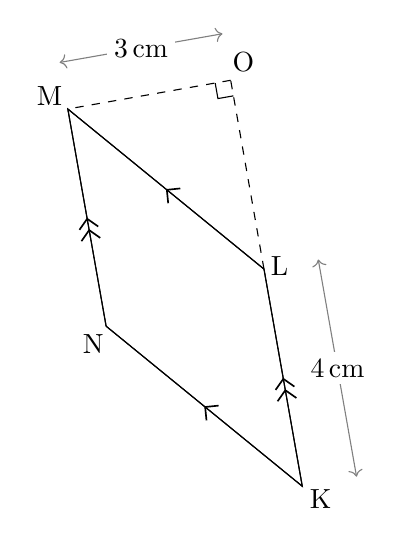
\begin{tikzpicture}[scale=1.0, baseline=(current bounding box.north)]
        \begin{scope}[rotate=100]

       \coordinate (K) at (0,0);
        \coordinate (L) at (2.8,0);
        \coordinate (O) at ($(L)+(2.434,0)$);  % extend out
        \coordinate (M) at ($(L)+(2.434,2.1)$); % Perpendicular upwards
        \coordinate (N) at ($(K)+(2.434,2.1)$); % Perpendicular upwards

        \draw (K)--(L)--(M)--(N)--cycle;
        \draw[dashed] (L)--(O);
        \draw[dashed] (O)--(M);

        \pic [draw, -, angle radius=0.2cm] {right angle=L--O--M};

        \draw[>=Straight Barb, postaction={decorate}, decoration={markings, mark=at position 0.5 with {\arrow[scale=1.5]{>>}}}] (K)--(L);
        \draw[>=Straight Barb, postaction={decorate}, decoration={markings, mark=at position 0.5 with {\arrow[scale=1.5]{>>}}}] (N)--(M);
        \draw[>=Straight Barb, postaction={decorate}, decoration={markings, mark=at position 0.5 with {\arrow[scale=1.5]{>}}}] (L)--(M);
        \draw[>=Straight Barb, postaction={decorate}, decoration={markings, mark=at position 0.5 with {\arrow[scale=1.5]{>}}}] (K)--(N);



        % Vertex LABELS
        % Labels relative to shape geometry
        \node at ($(K)+(-0.2,-0.2)$) {K};
        \node at ($(L)+(0.0,-0.2)$) {L};
        \node at ($(O)+(0.2,-0.2)$) {O};
        \node at ($(M)+(0.2,0.2)$) {M};
        \node at ($(N)+(-0.2,0.2)$) {N};


        % dotted/dashed arrows shifted away from edges
        % Horizontal side (A-B), shifted down yshift=0mm,
        \draw[<->, gray]
            ($(K) + (0,-0.7cm)$) -- ($(L) + (0,-0.7cm)$)
            node[black, midway, fill=white, inner sep=2.5pt] {4\,cm};

        % Vertical side (D-C), shifted right xshift=0mm,
        \draw[<->, gray]
            ($(O)+(0.6,0)$) -- ($(O |- M)+(0.6,0)$)
            node[black, midway, fill=white, inner sep=2.5pt] {3\,cm};

    \end{scope}
\end{tikzpicture}
\end{minipage}%
\hfill
\begin{minipage}{.4\textwidth}
  \begin{align*}
    \text{Area} &= \text{bh} \\
    \text{Area} &= 4 \text{cm} \times 3 \text{cm}  \\
    \text{Area} &= 12 \text{cm}^2
  \end{align*}
\end{minipage}

\par\vspace{1cm}\begin{minipage}{0.55\textwidth}
  \refstepcounter{minipagecount}
  \noindent{(\theminipagecount)}\quad
 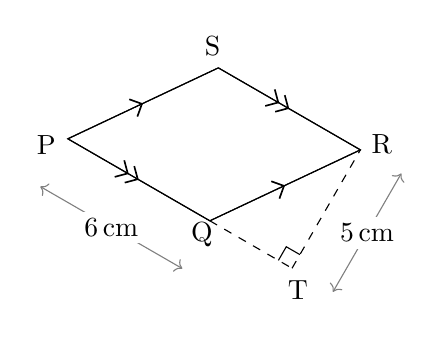
\begin{tikzpicture}[scale=1.0, baseline=(current bounding box.north)]
        \begin{scope}[rotate=-30]

       \coordinate (P) at (0,0);
        \coordinate (Q) at (2.083,0);
        \coordinate (T) at ($(Q)+(1.205,0)$);  % extend out
        \coordinate (R) at ($(Q)+(1.205,1.736)$); % Perpendicular upwards
        \coordinate (S) at ($(P)+(1.205,1.736)$); % Perpendicular upwards

        \draw (P)--(Q)--(R)--(S)--cycle;
        \draw[dashed] (Q)--(T);
        \draw[dashed] (T)--(R);

        \pic [draw, -, angle radius=0.2cm] {right angle=Q--T--R};

        \draw[>=Straight Barb, postaction={decorate}, decoration={markings, mark=at position 0.5 with {\arrow[scale=1.5]{>>}}}] (P)--(Q);
        \draw[>=Straight Barb, postaction={decorate}, decoration={markings, mark=at position 0.5 with {\arrow[scale=1.5]{>>}}}] (S)--(R);
        \draw[>=Straight Barb, postaction={decorate}, decoration={markings, mark=at position 0.5 with {\arrow[scale=1.5]{>}}}] (Q)--(R);
        \draw[>=Straight Barb, postaction={decorate}, decoration={markings, mark=at position 0.5 with {\arrow[scale=1.5]{>}}}] (P)--(S);



        % Vertex LABELS
        % Labels relative to shape geometry
        \node at ($(P)+(-0.2,-0.2)$) {P};
        \node at ($(Q)+(0.0,-0.2)$) {Q};
        \node at ($(T)+(0.2,-0.2)$) {T};
        \node at ($(R)+(0.2,0.2)$) {R};
        \node at ($(S)+(-0.2,0.2)$) {S};


        % dotted/dashed arrows shifted away from edges
        % Horizontal side (A-B), shifted down yshift=0mm,
        \draw[<->, gray]
            ($(P) + (0,-0.7cm)$) -- ($(Q) + (0,-0.7cm)$)
            node[black, midway, fill=white, inner sep=2.5pt] {6\,cm};

        % Vertical side (D-C), shifted right xshift=0mm,
        \draw[<->, gray]
            ($(T)+(0.6,0)$) -- ($(T |- R)+(0.6,0)$)
            node[black, midway, fill=white, inner sep=2.5pt] {5\,cm};

    \end{scope}
\end{tikzpicture}
\end{minipage}%
\hfill
\begin{minipage}{.4\textwidth}
  \begin{align*}
    \text{Area} &= \text{bh} \\
    \text{Area} &= 6 \text{cm} \times 5 \text{cm}  \\
    \text{Area} &= 30 \text{cm}^2
  \end{align*}
\end{minipage}

\par\vspace{1cm}\begin{minipage}{0.55\textwidth}
  \refstepcounter{minipagecount}
  \noindent{(\theminipagecount)}\quad
 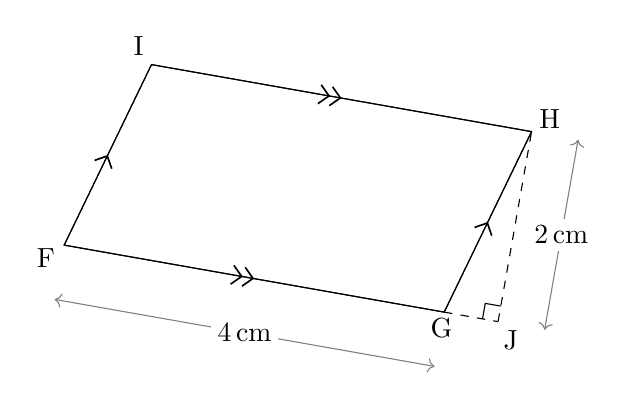
\begin{tikzpicture}[scale=1.0, baseline=(current bounding box.north)]
        \begin{scope}[rotate=-10]

       \coordinate (F) at (0,0);
        \coordinate (G) at (4.9,0);
        \coordinate (J) at ($(G)+(0.694,0)$);  % extend out
        \coordinate (H) at ($(G)+(0.694,2.45)$); % Perpendicular upwards
        \coordinate (I) at ($(F)+(0.694,2.45)$); % Perpendicular upwards

        \draw (F)--(G)--(H)--(I)--cycle;
        \draw[dashed] (G)--(J);
        \draw[dashed] (J)--(H);

        \pic [draw, -, angle radius=0.2cm] {right angle=G--J--H};

        \draw[>=Straight Barb, postaction={decorate}, decoration={markings, mark=at position 0.5 with {\arrow[scale=1.5]{>>}}}] (F)--(G);
        \draw[>=Straight Barb, postaction={decorate}, decoration={markings, mark=at position 0.5 with {\arrow[scale=1.5]{>>}}}] (I)--(H);
        \draw[>=Straight Barb, postaction={decorate}, decoration={markings, mark=at position 0.5 with {\arrow[scale=1.5]{>}}}] (G)--(H);
        \draw[>=Straight Barb, postaction={decorate}, decoration={markings, mark=at position 0.5 with {\arrow[scale=1.5]{>}}}] (F)--(I);



        % Vertex LABELS
        % Labels relative to shape geometry
        \node at ($(F)+(-0.2,-0.2)$) {F};
        \node at ($(G)+(0.0,-0.2)$) {G};
        \node at ($(J)+(0.2,-0.2)$) {J};
        \node at ($(H)+(0.2,0.2)$) {H};
        \node at ($(I)+(-0.2,0.2)$) {I};


        % dotted/dashed arrows shifted away from edges
        % Horizontal side (A-B), shifted down yshift=0mm,
        \draw[<->, gray]
            ($(F) + (0,-0.7cm)$) -- ($(G) + (0,-0.7cm)$)
            node[black, midway, fill=white, inner sep=2.5pt] {4\,cm};

        % Vertical side (D-C), shifted right xshift=0mm,
        \draw[<->, gray]
            ($(J)+(0.6,0)$) -- ($(J |- H)+(0.6,0)$)
            node[black, midway, fill=white, inner sep=2.5pt] {2\,cm};

    \end{scope}
\end{tikzpicture}
\end{minipage}%
\hfill
\begin{minipage}{.4\textwidth}
  \begin{align*}
    \text{Area} &= \text{bh} \\
    \text{Area} &= 4 \text{cm} \times 2 \text{cm}  \\
    \text{Area} &= 8 \text{cm}^2
  \end{align*}
\end{minipage}

\par\vspace{1cm}\begin{minipage}{0.55\textwidth}
  \refstepcounter{minipagecount}
  \noindent{(\theminipagecount)}\quad
 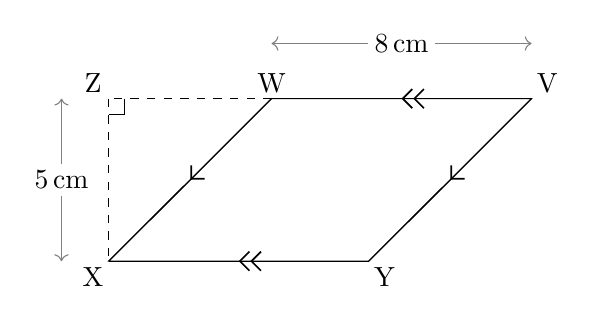
\begin{tikzpicture}[scale=1.0, baseline=(current bounding box.north)]
        \begin{scope}[rotate=180]

       \coordinate (V) at (0,0);
        \coordinate (W) at (3.302,0);
        \coordinate (Z) at ($(W)+(2.068,0)$);  % extend out
        \coordinate (X) at ($(W)+(2.068,2.064)$); % Perpendicular upwards
        \coordinate (Y) at ($(V)+(2.068,2.064)$); % Perpendicular upwards

        \draw (V)--(W)--(X)--(Y)--cycle;
        \draw[dashed] (W)--(Z);
        \draw[dashed] (Z)--(X);

        \pic [draw, -, angle radius=0.2cm] {right angle=W--Z--X};

        \draw[>=Straight Barb, postaction={decorate}, decoration={markings, mark=at position 0.5 with {\arrow[scale=1.5]{>>}}}] (V)--(W);
        \draw[>=Straight Barb, postaction={decorate}, decoration={markings, mark=at position 0.5 with {\arrow[scale=1.5]{>>}}}] (Y)--(X);
        \draw[>=Straight Barb, postaction={decorate}, decoration={markings, mark=at position 0.5 with {\arrow[scale=1.5]{>}}}] (W)--(X);
        \draw[>=Straight Barb, postaction={decorate}, decoration={markings, mark=at position 0.5 with {\arrow[scale=1.5]{>}}}] (V)--(Y);



        % Vertex LABELS
        % Labels relative to shape geometry
        \node at ($(V)+(-0.2,-0.2)$) {V};
        \node at ($(W)+(0.0,-0.2)$) {W};
        \node at ($(Z)+(0.2,-0.2)$) {Z};
        \node at ($(X)+(0.2,0.2)$) {X};
        \node at ($(Y)+(-0.2,0.2)$) {Y};


        % dotted/dashed arrows shifted away from edges
        % Horizontal side (A-B), shifted down yshift=0mm,
        \draw[<->, gray]
            ($(V) + (0,-0.7cm)$) -- ($(W) + (0,-0.7cm)$)
            node[black, midway, fill=white, inner sep=2.5pt] {8\,cm};

        % Vertical side (D-C), shifted right xshift=0mm,
        \draw[<->, gray]
            ($(Z)+(0.6,0)$) -- ($(Z |- X)+(0.6,0)$)
            node[black, midway, fill=white, inner sep=2.5pt] {5\,cm};

    \end{scope}
\end{tikzpicture}
\end{minipage}%
\hfill
\begin{minipage}{.4\textwidth}
  \begin{align*}
    \text{Area} &= \text{bh} \\
    \text{Area} &= 8 \text{cm} \times 5 \text{cm}  \\
    \text{Area} &= 40 \text{cm}^2
  \end{align*}
\end{minipage}

\par\vspace{1cm}\begin{minipage}{0.55\textwidth}
  \refstepcounter{minipagecount}
  \noindent{(\theminipagecount)}\quad
 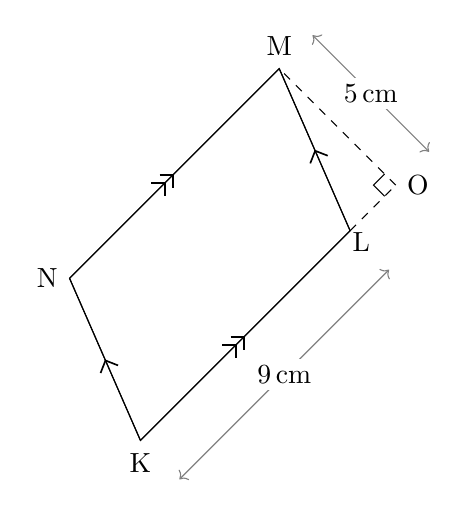
\begin{tikzpicture}[scale=1.0, baseline=(current bounding box.north)]
        \begin{scope}[rotate=45]

       \coordinate (K) at (0,0);
        \coordinate (L) at (3.766,0);
        \coordinate (O) at ($(L)+(0.819,0)$);  % extend out
        \coordinate (M) at ($(L)+(0.819,2.092)$); % Perpendicular upwards
        \coordinate (N) at ($(K)+(0.819,2.092)$); % Perpendicular upwards

        \draw (K)--(L)--(M)--(N)--cycle;
        \draw[dashed] (L)--(O);
        \draw[dashed] (O)--(M);

        \pic [draw, -, angle radius=0.2cm] {right angle=L--O--M};

        \draw[>=Straight Barb, postaction={decorate}, decoration={markings, mark=at position 0.5 with {\arrow[scale=1.5]{>>}}}] (K)--(L);
        \draw[>=Straight Barb, postaction={decorate}, decoration={markings, mark=at position 0.5 with {\arrow[scale=1.5]{>>}}}] (N)--(M);
        \draw[>=Straight Barb, postaction={decorate}, decoration={markings, mark=at position 0.5 with {\arrow[scale=1.5]{>}}}] (L)--(M);
        \draw[>=Straight Barb, postaction={decorate}, decoration={markings, mark=at position 0.5 with {\arrow[scale=1.5]{>}}}] (K)--(N);



        % Vertex LABELS
        % Labels relative to shape geometry
        \node at ($(K)+(-0.2,-0.2)$) {K};
        \node at ($(L)+(0.0,-0.2)$) {L};
        \node at ($(O)+(0.2,-0.2)$) {O};
        \node at ($(M)+(0.2,0.2)$) {M};
        \node at ($(N)+(-0.2,0.2)$) {N};


        % dotted/dashed arrows shifted away from edges
        % Horizontal side (A-B), shifted down yshift=0mm,
        \draw[<->, gray]
            ($(K) + (0,-0.7cm)$) -- ($(L) + (0,-0.7cm)$)
            node[black, midway, fill=white, inner sep=2.5pt] {9\,cm};

        % Vertical side (D-C), shifted right xshift=0mm,
        \draw[<->, gray]
            ($(O)+(0.6,0)$) -- ($(O |- M)+(0.6,0)$)
            node[black, midway, fill=white, inner sep=2.5pt] {5\,cm};

    \end{scope}
\end{tikzpicture}
\end{minipage}%
\hfill
\begin{minipage}{.4\textwidth}
  \begin{align*}
    \text{Area} &= \text{bh} \\
    \text{Area} &= 9 \text{cm} \times 5 \text{cm}  \\
    \text{Area} &= 45 \text{cm}^2
  \end{align*}
\end{minipage}

\par\vspace{1cm}\begin{minipage}{0.55\textwidth}
  \refstepcounter{minipagecount}
  \noindent{(\theminipagecount)}\quad
 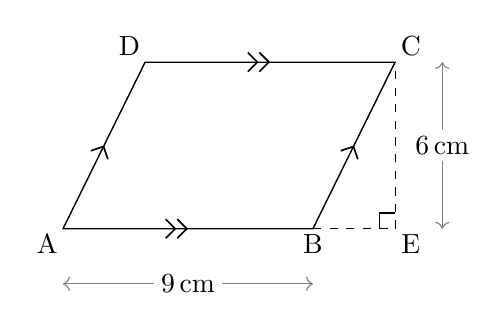
\begin{tikzpicture}[scale=1.0, baseline=(current bounding box.north)]
        \begin{scope}[rotate=0]

       \coordinate (A) at (0,0);
        \coordinate (B) at (3.174,0);
        \coordinate (E) at ($(B)+(1.043,0)$);  % extend out
        \coordinate (C) at ($(B)+(1.043,2.116)$); % Perpendicular upwards
        \coordinate (D) at ($(A)+(1.043,2.116)$); % Perpendicular upwards

        \draw (A)--(B)--(C)--(D)--cycle;
        \draw[dashed] (B)--(E);
        \draw[dashed] (E)--(C);

        \pic [draw, -, angle radius=0.2cm] {right angle=B--E--C};

        \draw[>=Straight Barb, postaction={decorate}, decoration={markings, mark=at position 0.5 with {\arrow[scale=1.5]{>>}}}] (A)--(B);
        \draw[>=Straight Barb, postaction={decorate}, decoration={markings, mark=at position 0.5 with {\arrow[scale=1.5]{>>}}}] (D)--(C);
        \draw[>=Straight Barb, postaction={decorate}, decoration={markings, mark=at position 0.5 with {\arrow[scale=1.5]{>}}}] (B)--(C);
        \draw[>=Straight Barb, postaction={decorate}, decoration={markings, mark=at position 0.5 with {\arrow[scale=1.5]{>}}}] (A)--(D);



        % Vertex LABELS
        % Labels relative to shape geometry
        \node at ($(A)+(-0.2,-0.2)$) {A};
        \node at ($(B)+(0.0,-0.2)$) {B};
        \node at ($(E)+(0.2,-0.2)$) {E};
        \node at ($(C)+(0.2,0.2)$) {C};
        \node at ($(D)+(-0.2,0.2)$) {D};


        % dotted/dashed arrows shifted away from edges
        % Horizontal side (A-B), shifted down yshift=0mm,
        \draw[<->, gray]
            ($(A) + (0,-0.7cm)$) -- ($(B) + (0,-0.7cm)$)
            node[black, midway, fill=white, inner sep=2.5pt] {9\,cm};

        % Vertical side (D-C), shifted right xshift=0mm,
        \draw[<->, gray]
            ($(E)+(0.6,0)$) -- ($(E |- C)+(0.6,0)$)
            node[black, midway, fill=white, inner sep=2.5pt] {6\,cm};

    \end{scope}
\end{tikzpicture}
\end{minipage}%
\hfill
\begin{minipage}{.4\textwidth}
  \begin{align*}
    \text{Area} &= \text{bh} \\
    \text{Area} &= 9 \text{cm} \times 6 \text{cm}  \\
    \text{Area} &= 54 \text{cm}^2
  \end{align*}
\end{minipage}

\par\vspace{1cm}\begin{minipage}{0.55\textwidth}
  \refstepcounter{minipagecount}
  \noindent{(\theminipagecount)}\quad
 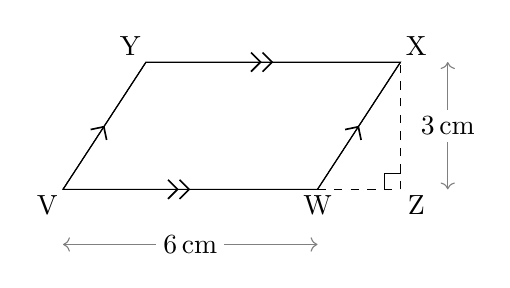
\begin{tikzpicture}[scale=1.0, baseline=(current bounding box.north)]
        \begin{scope}[rotate=0]

       \coordinate (V) at (0,0);
        \coordinate (W) at (3.232,0);
        \coordinate (Z) at ($(W)+(1.054,0)$);  % extend out
        \coordinate (X) at ($(W)+(1.054,1.616)$); % Perpendicular upwards
        \coordinate (Y) at ($(V)+(1.054,1.616)$); % Perpendicular upwards

        \draw (V)--(W)--(X)--(Y)--cycle;
        \draw[dashed] (W)--(Z);
        \draw[dashed] (Z)--(X);

        \pic [draw, -, angle radius=0.2cm] {right angle=W--Z--X};

        \draw[>=Straight Barb, postaction={decorate}, decoration={markings, mark=at position 0.5 with {\arrow[scale=1.5]{>>}}}] (V)--(W);
        \draw[>=Straight Barb, postaction={decorate}, decoration={markings, mark=at position 0.5 with {\arrow[scale=1.5]{>>}}}] (Y)--(X);
        \draw[>=Straight Barb, postaction={decorate}, decoration={markings, mark=at position 0.5 with {\arrow[scale=1.5]{>}}}] (W)--(X);
        \draw[>=Straight Barb, postaction={decorate}, decoration={markings, mark=at position 0.5 with {\arrow[scale=1.5]{>}}}] (V)--(Y);



        % Vertex LABELS
        % Labels relative to shape geometry
        \node at ($(V)+(-0.2,-0.2)$) {V};
        \node at ($(W)+(0.0,-0.2)$) {W};
        \node at ($(Z)+(0.2,-0.2)$) {Z};
        \node at ($(X)+(0.2,0.2)$) {X};
        \node at ($(Y)+(-0.2,0.2)$) {Y};


        % dotted/dashed arrows shifted away from edges
        % Horizontal side (A-B), shifted down yshift=0mm,
        \draw[<->, gray]
            ($(V) + (0,-0.7cm)$) -- ($(W) + (0,-0.7cm)$)
            node[black, midway, fill=white, inner sep=2.5pt] {6\,cm};

        % Vertical side (D-C), shifted right xshift=0mm,
        \draw[<->, gray]
            ($(Z)+(0.6,0)$) -- ($(Z |- X)+(0.6,0)$)
            node[black, midway, fill=white, inner sep=2.5pt] {3\,cm};

    \end{scope}
\end{tikzpicture}
\end{minipage}%
\hfill
\begin{minipage}{.4\textwidth}
  \begin{align*}
    \text{Area} &= \text{bh} \\
    \text{Area} &= 6 \text{cm} \times 3 \text{cm}  \\
    \text{Area} &= 18 \text{cm}^2
  \end{align*}
\end{minipage}

\par\vspace{1cm}\begin{minipage}{0.55\textwidth}
  \refstepcounter{minipagecount}
  \noindent{(\theminipagecount)}\quad
 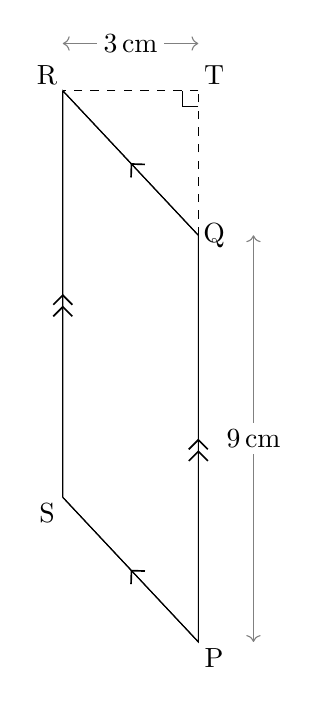
\begin{tikzpicture}[scale=1.0, baseline=(current bounding box.north)]
        \begin{scope}[rotate=90]

       \coordinate (P) at (0,0);
        \coordinate (Q) at (5.164,0);
        \coordinate (T) at ($(Q)+(1.836,0)$);  % extend out
        \coordinate (R) at ($(Q)+(1.836,1.721)$); % Perpendicular upwards
        \coordinate (S) at ($(P)+(1.836,1.721)$); % Perpendicular upwards

        \draw (P)--(Q)--(R)--(S)--cycle;
        \draw[dashed] (Q)--(T);
        \draw[dashed] (T)--(R);

        \pic [draw, -, angle radius=0.2cm] {right angle=Q--T--R};

        \draw[>=Straight Barb, postaction={decorate}, decoration={markings, mark=at position 0.5 with {\arrow[scale=1.5]{>>}}}] (P)--(Q);
        \draw[>=Straight Barb, postaction={decorate}, decoration={markings, mark=at position 0.5 with {\arrow[scale=1.5]{>>}}}] (S)--(R);
        \draw[>=Straight Barb, postaction={decorate}, decoration={markings, mark=at position 0.5 with {\arrow[scale=1.5]{>}}}] (Q)--(R);
        \draw[>=Straight Barb, postaction={decorate}, decoration={markings, mark=at position 0.5 with {\arrow[scale=1.5]{>}}}] (P)--(S);



        % Vertex LABELS
        % Labels relative to shape geometry
        \node at ($(P)+(-0.2,-0.2)$) {P};
        \node at ($(Q)+(0.0,-0.2)$) {Q};
        \node at ($(T)+(0.2,-0.2)$) {T};
        \node at ($(R)+(0.2,0.2)$) {R};
        \node at ($(S)+(-0.2,0.2)$) {S};


        % dotted/dashed arrows shifted away from edges
        % Horizontal side (A-B), shifted down yshift=0mm,
        \draw[<->, gray]
            ($(P) + (0,-0.7cm)$) -- ($(Q) + (0,-0.7cm)$)
            node[black, midway, fill=white, inner sep=2.5pt] {9\,cm};

        % Vertical side (D-C), shifted right xshift=0mm,
        \draw[<->, gray]
            ($(T)+(0.6,0)$) -- ($(T |- R)+(0.6,0)$)
            node[black, midway, fill=white, inner sep=2.5pt] {3\,cm};

    \end{scope}
\end{tikzpicture}
\end{minipage}%
\hfill
\begin{minipage}{.4\textwidth}
  \begin{align*}
    \text{Area} &= \text{bh} \\
    \text{Area} &= 9 \text{cm} \times 3 \text{cm}  \\
    \text{Area} &= 27 \text{cm}^2
  \end{align*}
\end{minipage}

\par\vspace{1cm}\begin{minipage}{0.55\textwidth}
  \refstepcounter{minipagecount}
  \noindent{(\theminipagecount)}\quad
 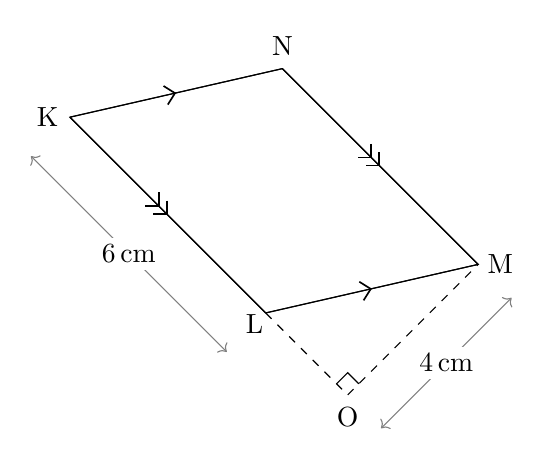
\begin{tikzpicture}[scale=1.0, baseline=(current bounding box.north)]
        \begin{scope}[rotate=315]

       \coordinate (K) at (0,0);
        \coordinate (L) at (3.516,0);
        \coordinate (O) at ($(L)+(1.472,0)$);  % extend out
        \coordinate (M) at ($(L)+(1.472,2.344)$); % Perpendicular upwards
        \coordinate (N) at ($(K)+(1.472,2.344)$); % Perpendicular upwards

        \draw (K)--(L)--(M)--(N)--cycle;
        \draw[dashed] (L)--(O);
        \draw[dashed] (O)--(M);

        \pic [draw, -, angle radius=0.2cm] {right angle=L--O--M};

        \draw[>=Straight Barb, postaction={decorate}, decoration={markings, mark=at position 0.5 with {\arrow[scale=1.5]{>>}}}] (K)--(L);
        \draw[>=Straight Barb, postaction={decorate}, decoration={markings, mark=at position 0.5 with {\arrow[scale=1.5]{>>}}}] (N)--(M);
        \draw[>=Straight Barb, postaction={decorate}, decoration={markings, mark=at position 0.5 with {\arrow[scale=1.5]{>}}}] (L)--(M);
        \draw[>=Straight Barb, postaction={decorate}, decoration={markings, mark=at position 0.5 with {\arrow[scale=1.5]{>}}}] (K)--(N);



        % Vertex LABELS
        % Labels relative to shape geometry
        \node at ($(K)+(-0.2,-0.2)$) {K};
        \node at ($(L)+(0.0,-0.2)$) {L};
        \node at ($(O)+(0.2,-0.2)$) {O};
        \node at ($(M)+(0.2,0.2)$) {M};
        \node at ($(N)+(-0.2,0.2)$) {N};


        % dotted/dashed arrows shifted away from edges
        % Horizontal side (A-B), shifted down yshift=0mm,
        \draw[<->, gray]
            ($(K) + (0,-0.7cm)$) -- ($(L) + (0,-0.7cm)$)
            node[black, midway, fill=white, inner sep=2.5pt] {6\,cm};

        % Vertical side (D-C), shifted right xshift=0mm,
        \draw[<->, gray]
            ($(O)+(0.6,0)$) -- ($(O |- M)+(0.6,0)$)
            node[black, midway, fill=white, inner sep=2.5pt] {4\,cm};

    \end{scope}
\end{tikzpicture}
\end{minipage}%
\hfill
\begin{minipage}{.4\textwidth}
  \begin{align*}
    \text{Area} &= \text{bh} \\
    \text{Area} &= 6 \text{cm} \times 4 \text{cm}  \\
    \text{Area} &= 24 \text{cm}^2
  \end{align*}
\end{minipage}

\par\vspace{1cm}\begin{minipage}{0.55\textwidth}
  \refstepcounter{minipagecount}
  \noindent{(\theminipagecount)}\quad
 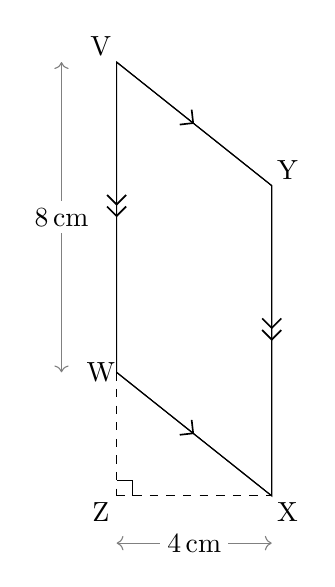
\begin{tikzpicture}[scale=1.0, baseline=(current bounding box.north)]
        \begin{scope}[rotate=270]

       \coordinate (V) at (0,0);
        \coordinate (W) at (3.94,0);
        \coordinate (Z) at ($(W)+(1.569,0)$);  % extend out
        \coordinate (X) at ($(W)+(1.569,1.97)$); % Perpendicular upwards
        \coordinate (Y) at ($(V)+(1.569,1.97)$); % Perpendicular upwards

        \draw (V)--(W)--(X)--(Y)--cycle;
        \draw[dashed] (W)--(Z);
        \draw[dashed] (Z)--(X);

        \pic [draw, -, angle radius=0.2cm] {right angle=W--Z--X};

        \draw[>=Straight Barb, postaction={decorate}, decoration={markings, mark=at position 0.5 with {\arrow[scale=1.5]{>>}}}] (V)--(W);
        \draw[>=Straight Barb, postaction={decorate}, decoration={markings, mark=at position 0.5 with {\arrow[scale=1.5]{>>}}}] (Y)--(X);
        \draw[>=Straight Barb, postaction={decorate}, decoration={markings, mark=at position 0.5 with {\arrow[scale=1.5]{>}}}] (W)--(X);
        \draw[>=Straight Barb, postaction={decorate}, decoration={markings, mark=at position 0.5 with {\arrow[scale=1.5]{>}}}] (V)--(Y);



        % Vertex LABELS
        % Labels relative to shape geometry
        \node at ($(V)+(-0.2,-0.2)$) {V};
        \node at ($(W)+(0.0,-0.2)$) {W};
        \node at ($(Z)+(0.2,-0.2)$) {Z};
        \node at ($(X)+(0.2,0.2)$) {X};
        \node at ($(Y)+(-0.2,0.2)$) {Y};


        % dotted/dashed arrows shifted away from edges
        % Horizontal side (A-B), shifted down yshift=0mm,
        \draw[<->, gray]
            ($(V) + (0,-0.7cm)$) -- ($(W) + (0,-0.7cm)$)
            node[black, midway, fill=white, inner sep=2.5pt] {8\,cm};

        % Vertical side (D-C), shifted right xshift=0mm,
        \draw[<->, gray]
            ($(Z)+(0.6,0)$) -- ($(Z |- X)+(0.6,0)$)
            node[black, midway, fill=white, inner sep=2.5pt] {4\,cm};

    \end{scope}
\end{tikzpicture}
\end{minipage}%
\hfill
\begin{minipage}{.4\textwidth}
  \begin{align*}
    \text{Area} &= \text{bh} \\
    \text{Area} &= 8 \text{cm} \times 4 \text{cm}  \\
    \text{Area} &= 32 \text{cm}^2
  \end{align*}
\end{minipage}

\par\vspace{1cm}\begin{minipage}{0.55\textwidth}
  \refstepcounter{minipagecount}
  \noindent{(\theminipagecount)}\quad
 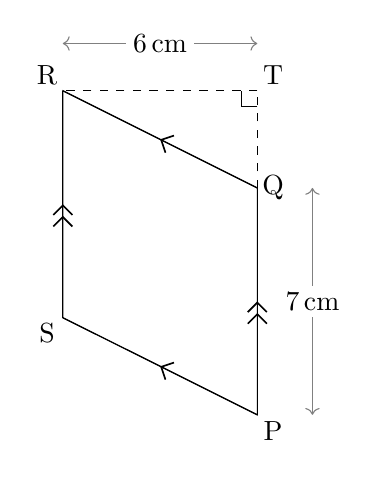
\begin{tikzpicture}[scale=1.0, baseline=(current bounding box.north)]
        \begin{scope}[rotate=90]

       \coordinate (P) at (0,0);
        \coordinate (Q) at (2.882,0);
        \coordinate (T) at ($(Q)+(1.234,0)$);  % extend out
        \coordinate (R) at ($(Q)+(1.234,2.47)$); % Perpendicular upwards
        \coordinate (S) at ($(P)+(1.234,2.47)$); % Perpendicular upwards

        \draw (P)--(Q)--(R)--(S)--cycle;
        \draw[dashed] (Q)--(T);
        \draw[dashed] (T)--(R);

        \pic [draw, -, angle radius=0.2cm] {right angle=Q--T--R};

        \draw[>=Straight Barb, postaction={decorate}, decoration={markings, mark=at position 0.5 with {\arrow[scale=1.5]{>>}}}] (P)--(Q);
        \draw[>=Straight Barb, postaction={decorate}, decoration={markings, mark=at position 0.5 with {\arrow[scale=1.5]{>>}}}] (S)--(R);
        \draw[>=Straight Barb, postaction={decorate}, decoration={markings, mark=at position 0.5 with {\arrow[scale=1.5]{>}}}] (Q)--(R);
        \draw[>=Straight Barb, postaction={decorate}, decoration={markings, mark=at position 0.5 with {\arrow[scale=1.5]{>}}}] (P)--(S);



        % Vertex LABELS
        % Labels relative to shape geometry
        \node at ($(P)+(-0.2,-0.2)$) {P};
        \node at ($(Q)+(0.0,-0.2)$) {Q};
        \node at ($(T)+(0.2,-0.2)$) {T};
        \node at ($(R)+(0.2,0.2)$) {R};
        \node at ($(S)+(-0.2,0.2)$) {S};


        % dotted/dashed arrows shifted away from edges
        % Horizontal side (A-B), shifted down yshift=0mm,
        \draw[<->, gray]
            ($(P) + (0,-0.7cm)$) -- ($(Q) + (0,-0.7cm)$)
            node[black, midway, fill=white, inner sep=2.5pt] {7\,cm};

        % Vertical side (D-C), shifted right xshift=0mm,
        \draw[<->, gray]
            ($(T)+(0.6,0)$) -- ($(T |- R)+(0.6,0)$)
            node[black, midway, fill=white, inner sep=2.5pt] {6\,cm};

    \end{scope}
\end{tikzpicture}
\end{minipage}%
\hfill
\begin{minipage}{.4\textwidth}
  \begin{align*}
    \text{Area} &= \text{bh} \\
    \text{Area} &= 7 \text{cm} \times 6 \text{cm}  \\
    \text{Area} &= 42 \text{cm}^2
  \end{align*}
\end{minipage}

\par\vspace{1cm}\begin{minipage}{0.55\textwidth}
  \refstepcounter{minipagecount}
  \noindent{(\theminipagecount)}\quad
 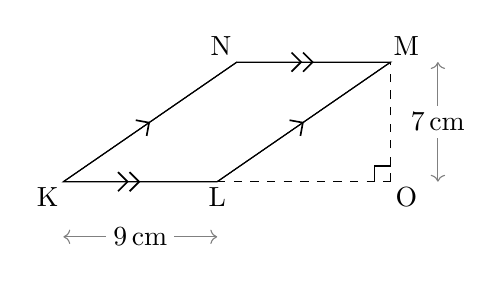
\begin{tikzpicture}[scale=1.0, baseline=(current bounding box.north)]
        \begin{scope}[rotate=0]

       \coordinate (K) at (0,0);
        \coordinate (L) at (1.953,0);
        \coordinate (O) at ($(L)+(2.203,0)$);  % extend out
        \coordinate (M) at ($(L)+(2.203,1.519)$); % Perpendicular upwards
        \coordinate (N) at ($(K)+(2.203,1.519)$); % Perpendicular upwards

        \draw (K)--(L)--(M)--(N)--cycle;
        \draw[dashed] (L)--(O);
        \draw[dashed] (O)--(M);

        \pic [draw, -, angle radius=0.2cm] {right angle=L--O--M};

        \draw[>=Straight Barb, postaction={decorate}, decoration={markings, mark=at position 0.5 with {\arrow[scale=1.5]{>>}}}] (K)--(L);
        \draw[>=Straight Barb, postaction={decorate}, decoration={markings, mark=at position 0.5 with {\arrow[scale=1.5]{>>}}}] (N)--(M);
        \draw[>=Straight Barb, postaction={decorate}, decoration={markings, mark=at position 0.5 with {\arrow[scale=1.5]{>}}}] (L)--(M);
        \draw[>=Straight Barb, postaction={decorate}, decoration={markings, mark=at position 0.5 with {\arrow[scale=1.5]{>}}}] (K)--(N);



        % Vertex LABELS
        % Labels relative to shape geometry
        \node at ($(K)+(-0.2,-0.2)$) {K};
        \node at ($(L)+(0.0,-0.2)$) {L};
        \node at ($(O)+(0.2,-0.2)$) {O};
        \node at ($(M)+(0.2,0.2)$) {M};
        \node at ($(N)+(-0.2,0.2)$) {N};


        % dotted/dashed arrows shifted away from edges
        % Horizontal side (A-B), shifted down yshift=0mm,
        \draw[<->, gray]
            ($(K) + (0,-0.7cm)$) -- ($(L) + (0,-0.7cm)$)
            node[black, midway, fill=white, inner sep=2.5pt] {9\,cm};

        % Vertical side (D-C), shifted right xshift=0mm,
        \draw[<->, gray]
            ($(O)+(0.6,0)$) -- ($(O |- M)+(0.6,0)$)
            node[black, midway, fill=white, inner sep=2.5pt] {7\,cm};

    \end{scope}
\end{tikzpicture}
\end{minipage}%
\hfill
\begin{minipage}{.4\textwidth}
  \begin{align*}
    \text{Area} &= \text{bh} \\
    \text{Area} &= 9 \text{cm} \times 7 \text{cm}  \\
    \text{Area} &= 63 \text{cm}^2
  \end{align*}
\end{minipage}

\par\vspace{1cm}\begin{minipage}{0.55\textwidth}
  \refstepcounter{minipagecount}
  \noindent{(\theminipagecount)}\quad
 \begin{tikzpicture}[scale=1.0, baseline=(current bounding box.north)]
        \begin{scope}[rotate=225]

       \coordinate (V) at (0,0);
        \coordinate (W) at (4.747,0);
        \coordinate (Z) at ($(W)+(1.986,0)$);  % extend out
        \coordinate (X) at ($(W)+(1.986,1.78)$); % Perpendicular upwards
        \coordinate (Y) at ($(V)+(1.986,1.78)$); % Perpendicular upwards

        \draw (V)--(W)--(X)--(Y)--cycle;
        \draw[dashed] (W)--(Z);
        \draw[dashed] (Z)--(X);

        \pic [draw, -, angle radius=0.2cm] {right angle=W--Z--X};

        \draw[>=Straight Barb, postaction={decorate}, decoration={markings, mark=at position 0.5 with {\arrow[scale=1.5]{>>}}}] (V)--(W);
        \draw[>=Straight Barb, postaction={decorate}, decoration={markings, mark=at position 0.5 with {\arrow[scale=1.5]{>>}}}] (Y)--(X);
        \draw[>=Straight Barb, postaction={decorate}, decoration={markings, mark=at position 0.5 with {\arrow[scale=1.5]{>}}}] (W)--(X);
        \draw[>=Straight Barb, postaction={decorate}, decoration={markings, mark=at position 0.5 with {\arrow[scale=1.5]{>}}}] (V)--(Y);



        % Vertex LABELS
        % Labels relative to shape geometry
        \node at ($(V)+(-0.2,-0.2)$) {V};
        \node at ($(W)+(0.0,-0.2)$) {W};
        \node at ($(Z)+(0.2,-0.2)$) {Z};
        \node at ($(X)+(0.2,0.2)$) {X};
        \node at ($(Y)+(-0.2,0.2)$) {Y};


        % dotted/dashed arrows shifted away from edges
        % Horizontal side (A-B), shifted down yshift=0mm,
        \draw[<->, gray]
            ($(V) + (0,-0.7cm)$) -- ($(W) + (0,-0.7cm)$)
            node[black, midway, fill=white, inner sep=2.5pt] {8\,cm};

        % Vertical side (D-C), shifted right xshift=0mm,
        \draw[<->, gray]
            ($(Z)+(0.6,0)$) -- ($(Z |- X)+(0.6,0)$)
            node[black, midway, fill=white, inner sep=2.5pt] {3\,cm};

    \end{scope}
\end{tikzpicture}
\end{minipage}%
\hfill
\begin{minipage}{.4\textwidth}
  \begin{align*}
    \text{Area} &= \text{bh} \\
    \text{Area} &= 8 \text{cm} \times 3 \text{cm}  \\
    \text{Area} &= 24 \text{cm}^2
  \end{align*}
\end{minipage}

\par\vspace{1cm}\begin{minipage}{0.55\textwidth}
  \refstepcounter{minipagecount}
  \noindent{(\theminipagecount)}\quad
 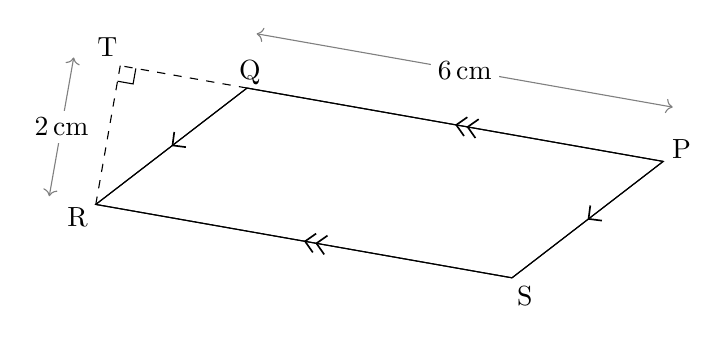
\begin{tikzpicture}[scale=1.0, baseline=(current bounding box.north)]
        \begin{scope}[rotate=170]

       \coordinate (P) at (0,0);
        \coordinate (Q) at (5.366,0);
        \coordinate (T) at ($(Q)+(1.634,0)$);  % extend out
        \coordinate (R) at ($(Q)+(1.634,1.789)$); % Perpendicular upwards
        \coordinate (S) at ($(P)+(1.634,1.789)$); % Perpendicular upwards

        \draw (P)--(Q)--(R)--(S)--cycle;
        \draw[dashed] (Q)--(T);
        \draw[dashed] (T)--(R);

        \pic [draw, -, angle radius=0.2cm] {right angle=Q--T--R};

        \draw[>=Straight Barb, postaction={decorate}, decoration={markings, mark=at position 0.5 with {\arrow[scale=1.5]{>>}}}] (P)--(Q);
        \draw[>=Straight Barb, postaction={decorate}, decoration={markings, mark=at position 0.5 with {\arrow[scale=1.5]{>>}}}] (S)--(R);
        \draw[>=Straight Barb, postaction={decorate}, decoration={markings, mark=at position 0.5 with {\arrow[scale=1.5]{>}}}] (Q)--(R);
        \draw[>=Straight Barb, postaction={decorate}, decoration={markings, mark=at position 0.5 with {\arrow[scale=1.5]{>}}}] (P)--(S);



        % Vertex LABELS
        % Labels relative to shape geometry
        \node at ($(P)+(-0.2,-0.2)$) {P};
        \node at ($(Q)+(0.0,-0.2)$) {Q};
        \node at ($(T)+(0.2,-0.2)$) {T};
        \node at ($(R)+(0.2,0.2)$) {R};
        \node at ($(S)+(-0.2,0.2)$) {S};


        % dotted/dashed arrows shifted away from edges
        % Horizontal side (A-B), shifted down yshift=0mm,
        \draw[<->, gray]
            ($(P) + (0,-0.7cm)$) -- ($(Q) + (0,-0.7cm)$)
            node[black, midway, fill=white, inner sep=2.5pt] {6\,cm};

        % Vertical side (D-C), shifted right xshift=0mm,
        \draw[<->, gray]
            ($(T)+(0.6,0)$) -- ($(T |- R)+(0.6,0)$)
            node[black, midway, fill=white, inner sep=2.5pt] {2\,cm};

    \end{scope}
\end{tikzpicture}
\end{minipage}%
\hfill
\begin{minipage}{.4\textwidth}
  \begin{align*}
    \text{Area} &= \text{bh} \\
    \text{Area} &= 6 \text{cm} \times 2 \text{cm}  \\
    \text{Area} &= 12 \text{cm}^2
  \end{align*}
\end{minipage}

\par\vspace{1cm}\begin{minipage}{0.55\textwidth}
  \refstepcounter{minipagecount}
  \noindent{(\theminipagecount)}\quad
 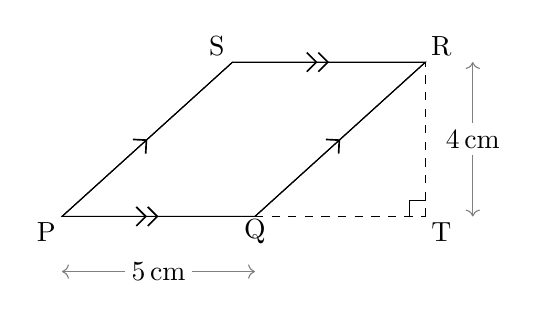
\begin{tikzpicture}[scale=1.0, baseline=(current bounding box.north)]
        \begin{scope}[rotate=0]

       \coordinate (P) at (0,0);
        \coordinate (Q) at (2.45,0);
        \coordinate (T) at ($(Q)+(2.166,0)$);  % extend out
        \coordinate (R) at ($(Q)+(2.166,1.96)$); % Perpendicular upwards
        \coordinate (S) at ($(P)+(2.166,1.96)$); % Perpendicular upwards

        \draw (P)--(Q)--(R)--(S)--cycle;
        \draw[dashed] (Q)--(T);
        \draw[dashed] (T)--(R);

        \pic [draw, -, angle radius=0.2cm] {right angle=Q--T--R};

        \draw[>=Straight Barb, postaction={decorate}, decoration={markings, mark=at position 0.5 with {\arrow[scale=1.5]{>>}}}] (P)--(Q);
        \draw[>=Straight Barb, postaction={decorate}, decoration={markings, mark=at position 0.5 with {\arrow[scale=1.5]{>>}}}] (S)--(R);
        \draw[>=Straight Barb, postaction={decorate}, decoration={markings, mark=at position 0.5 with {\arrow[scale=1.5]{>}}}] (Q)--(R);
        \draw[>=Straight Barb, postaction={decorate}, decoration={markings, mark=at position 0.5 with {\arrow[scale=1.5]{>}}}] (P)--(S);



        % Vertex LABELS
        % Labels relative to shape geometry
        \node at ($(P)+(-0.2,-0.2)$) {P};
        \node at ($(Q)+(0.0,-0.2)$) {Q};
        \node at ($(T)+(0.2,-0.2)$) {T};
        \node at ($(R)+(0.2,0.2)$) {R};
        \node at ($(S)+(-0.2,0.2)$) {S};


        % dotted/dashed arrows shifted away from edges
        % Horizontal side (A-B), shifted down yshift=0mm,
        \draw[<->, gray]
            ($(P) + (0,-0.7cm)$) -- ($(Q) + (0,-0.7cm)$)
            node[black, midway, fill=white, inner sep=2.5pt] {5\,cm};

        % Vertical side (D-C), shifted right xshift=0mm,
        \draw[<->, gray]
            ($(T)+(0.6,0)$) -- ($(T |- R)+(0.6,0)$)
            node[black, midway, fill=white, inner sep=2.5pt] {4\,cm};

    \end{scope}
\end{tikzpicture}
\end{minipage}%
\hfill
\begin{minipage}{.4\textwidth}
  \begin{align*}
    \text{Area} &= \text{bh} \\
    \text{Area} &= 5 \text{cm} \times 4 \text{cm}  \\
    \text{Area} &= 20 \text{cm}^2
  \end{align*}
\end{minipage}

\par\vspace{1cm}\begin{minipage}{0.55\textwidth}
  \refstepcounter{minipagecount}
  \noindent{(\theminipagecount)}\quad
 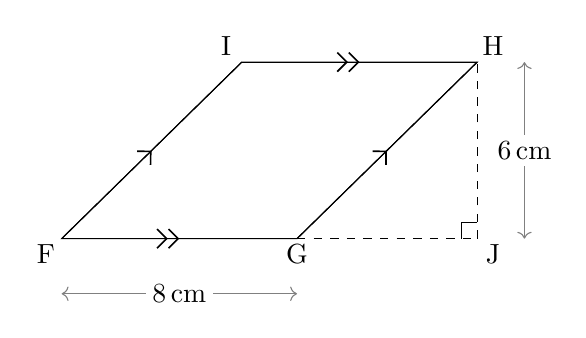
\begin{tikzpicture}[scale=1.0, baseline=(current bounding box.north)]
        \begin{scope}[rotate=0]

       \coordinate (F) at (0,0);
        \coordinate (G) at (2.989,0);
        \coordinate (J) at ($(G)+(2.288,0)$);  % extend out
        \coordinate (H) at ($(G)+(2.288,2.242)$); % Perpendicular upwards
        \coordinate (I) at ($(F)+(2.288,2.242)$); % Perpendicular upwards

        \draw (F)--(G)--(H)--(I)--cycle;
        \draw[dashed] (G)--(J);
        \draw[dashed] (J)--(H);

        \pic [draw, -, angle radius=0.2cm] {right angle=G--J--H};

        \draw[>=Straight Barb, postaction={decorate}, decoration={markings, mark=at position 0.5 with {\arrow[scale=1.5]{>>}}}] (F)--(G);
        \draw[>=Straight Barb, postaction={decorate}, decoration={markings, mark=at position 0.5 with {\arrow[scale=1.5]{>>}}}] (I)--(H);
        \draw[>=Straight Barb, postaction={decorate}, decoration={markings, mark=at position 0.5 with {\arrow[scale=1.5]{>}}}] (G)--(H);
        \draw[>=Straight Barb, postaction={decorate}, decoration={markings, mark=at position 0.5 with {\arrow[scale=1.5]{>}}}] (F)--(I);



        % Vertex LABELS
        % Labels relative to shape geometry
        \node at ($(F)+(-0.2,-0.2)$) {F};
        \node at ($(G)+(0.0,-0.2)$) {G};
        \node at ($(J)+(0.2,-0.2)$) {J};
        \node at ($(H)+(0.2,0.2)$) {H};
        \node at ($(I)+(-0.2,0.2)$) {I};


        % dotted/dashed arrows shifted away from edges
        % Horizontal side (A-B), shifted down yshift=0mm,
        \draw[<->, gray]
            ($(F) + (0,-0.7cm)$) -- ($(G) + (0,-0.7cm)$)
            node[black, midway, fill=white, inner sep=2.5pt] {8\,cm};

        % Vertical side (D-C), shifted right xshift=0mm,
        \draw[<->, gray]
            ($(J)+(0.6,0)$) -- ($(J |- H)+(0.6,0)$)
            node[black, midway, fill=white, inner sep=2.5pt] {6\,cm};

    \end{scope}
\end{tikzpicture}
\end{minipage}%
\hfill
\begin{minipage}{.4\textwidth}
  \begin{align*}
    \text{Area} &= \text{bh} \\
    \text{Area} &= 8 \text{cm} \times 6 \text{cm}  \\
    \text{Area} &= 48 \text{cm}^2
  \end{align*}
\end{minipage}

\par\vspace{1cm}

\end{document}
